%%%%%%%%%%%%
%
% $Autor: Wings $
% $Datum: 2019-03-05 08:03:15Z $
% $Pfad: LEDBuiltIn $
% $Version: 4250 $
% !TeX spellcheck = en_GB/de_DE
% !TeX encoding = utf8
% !TeX root = filename 
% !TeX TXS-program:bibliography = txs:///biber
%
%%%%%%%%%%%%

%todo citations
%todo create tikz pictures
%todo test the code


\chapter{Built-inLED}\index{LED!Built-in LED}

Some Arduino boards have a LED on board which can use for the application. \cite{ArduinoNanoGetStarted:2024,Arduino:2023a,Arduino:2023}

\section{General Information}

LEDs are used in the applications. Depending on the action performed by a user or the sketch, corresponding feedback can be provided. This can take the form of the LED switching on, switching off or flashing. \cite{Kurniawan:2021b}




\section{Built-in LED}

The built-in LED of the Arduino Nano 33 BLE Sense is a single orange LED that is connected to pin 13 on the board. The built-in LED is active-high, which means that setting the pin to \PYTHON{HIGH} will turn the LED on, and setting the pin to \PYTHON{LOW} will turn the LED off. The built-in LED can be used for various purposes, such as indicating the status of the board, displaying sensor data, creating visual effects, or debugging. \cite{Arduino:2023a,Arduino:2023,ArduinoNano33Manual:2022}


\bigskip



\begin{center}    
    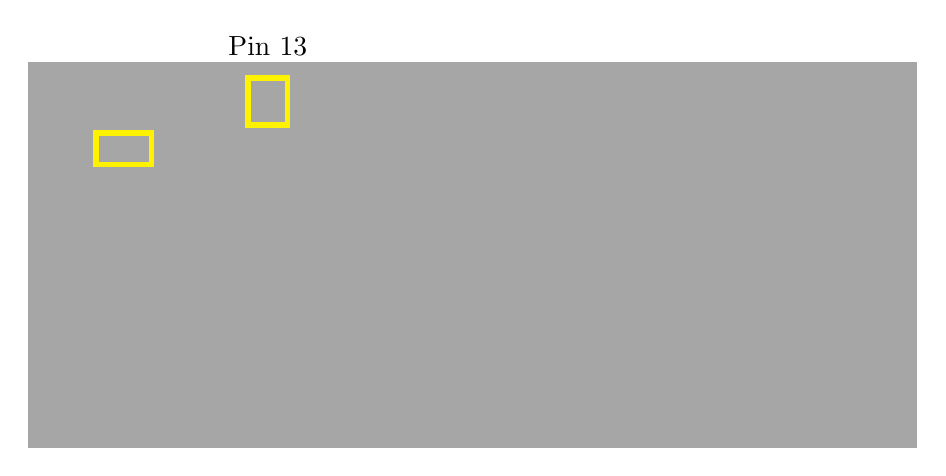
\begin{tikzpicture}
        %\node at (0,0) (Board) {\includegraphics{Arduino/Nano33BLE/Nano33BLESense}};
        
        \ArduinoNanoTikz;
        
        \fill[gray, opacity=0.7] (-11.2,-0.2) rectangle (0.1,4.7);
        
        \coordinate (A) at (-10.33,3.4);
        \coordinate (B) at (-9.63,3.8); 
           
        
        \coordinate (C) at (-8.4,3.9);
        \coordinate (D) at (-7.9,4.5);  
        
        \def\cliparea{(C) rectangle (D); (A) rectangle (B); }  
        
        \begin{scope}
          \clip (A) rectangle (B);
            
            \ArduinoNanoTikz
            
            %\node at (0,0) (Board) {\includegraphics{Arduino/Nano33BLE/Nano33BLESense}};
            
        \end{scope}
    
%        \fill[ArduinoColor] (C) rectangle (D);
%         \fill[gray!30] ({-8.16-0.195},4.145) rectangle ++(0.39, 0.39); 
%        \draw[fill=gray!30,gray!30] (-8.145,4.143) circle(0.195); 
%        \draw[fill=gray!60,gray!60] (-8.145,4.143) circle(0.165); 
%        \fill[white,white](-8.145,{4.143+0.39}) circle (0.1275);
        
        \draw[yellow,line width=2pt] (A)  rectangle (B);
        \draw[yellow,line width=2pt] (C)  rectangle (D);
        
        \node (P25) at (-8.15, 4.9) {Pin 13};
    \end{tikzpicture}    
  
 

  \captionof{figure}{Arduino Nano 33 BLE Sense's built-in LED  with Pin 13}  
\end{center}
    

\section{Specification}

\subsection{Pin Assignment}

The built-in LED is a orange LED and connected to pin 13.\index{Pin!Pin 13} The brightness can not be controlled. \cite{Arduino:2023a,Arduino:2023}

\begin{description}
    \item [Built-in LED:] \PYTHON{LED\_BUILTIN =  13u}
\end{description}

Built-in LED is active-high and connected to pin 13.

The built-in LED can be controlled programmatically by setting the pin to \PYTHON{HIGH} or \PYTHON{LOW}. 


%\Mynote{cite data sheet, power consumption?}

The pin 13 must be defined as an output in the function \PYTHON{setup} by setting \PYTHON{pinMode (13, OUTPUT)}, otherwise the LED cannot be switched on.

\medskip 


The pin 13 can also be used otherwise. Then the LED is not in use.

%\Mynote{What happen if there is another LED at the pin? Both in use?}


\subsection{Power Comsumption}

The power comsumption has to be considered. It is the same value as for the power LED, see section~\ref{LEDPowerComsumption}.


%\section{Calibration}
%
%cite method

\section{Simple Code}

\subsection{Simple Code for the Built-in LED}

For using the built-in LED, a simple library is introduced here.

\medskip


In the header file \FILE{BuiltinLED.h}, see code \ref{Nano:BuiltinLEDHeader}, are the declaration of the variables and the  functions. A variable is connected to pin 13.\index{Pin!Pin 13} The pin 13 is defined as an output in the function \PYTHON{BuiltinLEDinit}. There are  2 functions:

\begin{enumerate}
    \item \PYTHON{BuiltinLEDinit}: This funtion initializes the digital pin 13 of the built-in LED as an output.
    \item \PYTHON{BuiltinLED}: This funtion switches the built-in LED  on or off.
\end{enumerate}

{
    \captionof{code}{Header file without comments for using the Built-in LED}\label{Nano:BultinLEDHeader}
    \ArduinoExternal{linerange={9-14,27-28,40-42}}{../../Code/Nano33BLESense/LEDs/BuiltinLED.h}
}

In the file \FILE{BuiltinLED.cpp}, see code \ref{Nano:BuiltinLEDCpp}, the functions are implemented.

{
  \captionof{code}{Code file without comments for using the Built-in LED}\label{Nano:BuiltinLEDCpp}
  \ArduinoExternal{linerange={12-15,28-34,46-51}}{../../Code/Nano33BLESense/LEDs/builtinLED.cpp}
}


\subsection{Simple Code for Testing the Built-in LED}

In the sketch \ref{Nano:BuiltinLEDTest}, a variable is connected to pin 13.\index{Pin!Pin 13} The pin is defined as an output in the function \PYTHON{setup}. In the function \PYTHON{loop}, the LED is switched on for 1 second and switched off for 1 second so that the LED flashes accordingly.



{
  \captionof{code}{Simple sketch without comments to control the built-in LED}\label{Nano:BuiltinLEDTest}
  \ArduinoExternal{linerange={17-19,31-34,47-57}}{../../Code/Nano33BLESense/Test/TestLEDBuiltin.ino}
}

\bigskip

This is just a simple example. The variable \PYTHON{LED\_BUILTIN} is already defined, so the assignment is not necessary. The command \PYTHON{delay} should be avoided in an Arduino sketch. Instead, variables of the type \PYTHON{elapsedMillis} should be used.

%\Mynote{Arduino Referenz \url{https://github.com/pfeerick/elapsedMillis/wiki}}

\section{Tests}

\subsection{Simple Function Test}

The simplest test is the flashing of the LED at 2 Hz, see sketch \ref{Nano:BuiltinLEDTest2}.

{
  \captionof{code}{Simple sketch to test the built-in LED}\label{Nano:BuiltinLEDTest2}
  \ArduinoExternal{linerange={17-19,31-34,47-57}}{../../Code/Nano33BLESense/Test/TestLEDBuiltin.ino}
}


\subsection{Test all Functions}

As the built-in does not allow any special manipulations, all functions are covered with the sketch \ref{Nano:BuiltinLEDTest2}.

\section{Simple Application}

In many applications, it is necessary to save power so that the LED is not switched on continuously. Nevertheless, feedback is required as to whether the system, e.g. a fire detector, is switched on and functional. In this case, the LED is switched on for 1 second at a defined time interval, in this case 30 seconds. This is implemented in the example \ref{Nano:TestBuiltinApp}.

{
    \captionof{code}{A simple watch dog: A simple watchdog: the built-in LED is switched on for 1 second every 30 seconds.}\label{Nano:TestBuiltinApp}
    \ArduinoExternal{linerange={13-22,35-43,56-62}}{../../Code/Nano33BLESense/Test/TestLEDBuiltinApplication.ino}
}



\section{Further Readings}

\begin{itemize}
    \item Babu, Neelakandan Ramesh and  Chenchireddy, Kalagotla and  Reddy, V. Harsha Vardhan and  Samhitha, Dr. and Apparao, P. and  Kalyan, Ch. Pavan: \textsl{Case Study on Ni-MH Battery}. 2023 2\textsuperscript{nd} International Conference on Applied Artificial Intelligence and Computing (ICAAIC), 2023. \cite{Babu:2023}
    \item Scherer, Thomas: \textsl{Elektor special: Stromversorgung und Batterien}. Elektor Special. 2022. \cite{Scherer:2022}
\end{itemize}



